\chapter[Extraction of RDF Knowledge from Templated Websites]{REX: Web-Scale Extension of RDF Knowledge Bases from Templated Websites}
\label{cha:rex}
\graffito{This chapter introduces REX, a Web-scale extraction framework for semantic data from templated websites which was presented in~\cite{rex}. The author of this thesis was one of the two main authors of the corresponding publication~\cite{rex} together with Lorenz Bühmann. He co-designed the approach and implemented the storage, crawling and entity linking parts of the pipeline as well a evaluated this approach programmatically and manually.}



The \ac{LOD} Cloud has grown from 12 datasets to over 2000 knowledge bases in less than 10 years.\footnote{\url{http://stats.lod2.eu/}}
%The amount of data now available on the LOD Cloud exceeds 31 billion triples, which pertain to domains as diverse as movies, music, sports, bio-medicine and many others. 
This steady growth of the \ac{LOD} Cloud promises to continue as very large datasets such as  Linked TCGA~\cite{SAL+13a} with 20.4 billion triples are added to it. 
However, the \ac{LOD} Cloud still contains only a fraction of the knowledge available on the Web~\cite{GER+13}. 
This lack of coverage is mainly due to the way the data available on the \ac{LOD} Cloud is extracted. 

Most commonly, the data in the \ac{LOD} Cloud originates from one of two types of sources: structured data (especially databases such as Drugbank,\footnote{\url{http://www.drugbank.ca}} Diseasome,\footnote{\url{http://diseasome.eu}} etc.)~and semi-structured data sources, e.g., data extracted from the Wikipedia\footnote{\url{http://wikipedia.org}} infoboxes. 
Furthermore, approaches like CETUS (Chapter~\ref{cha:cetus} and  AGDISTIS (Chapter~\ref{cha:agdistis} provide further means to extract high-quality \ac{RDF} data from unstructured text but are not yet widely to construct \ac{KB}s.

While generating \ac{RDF} triples from structured data (especially databases) is well supported by systems such as Triplify~\cite{triplify_www}, D2R~\cite{Bizer04} and SPARQLMap~\cite{unbehauen-jist-2012-sparqlmap}
, devising automatic means to generate \ac{RDF} from semi-structured data is a more challenging  problem. 
Currently, this challenge is addressed by ad-hoc or manual (e.g., community-driven) solutions. 
For example, the well-known DBpedia~\cite{dbpedia-swj} provides a mapping wiki\footnote{\url{http://mappings.dbpedia.org}} where users can explicate how the content of infoboxes is to be transformed into \ac{RDF}. 
On the one hand, manual approaches offer the advantage of leading to high-precision data; on the other hand, they suffer of a limited recall because of the small number of Web sources from which the data is extracted. 
For example, DBpedia only contains a fraction of the movies that were published over the last years because it was extracted exclusively from Wikipedia.
%\footnote{\url{http://wikipedia.org}} 
Moreover, the same  \ac{KB} only contains a fraction of the cast of some of the movies it describes.

The main aim of this paper is to address the challenge of extracting \ac{RDF} from semi-structured data.
We introduce REX, an open-source framework for the extraction of \ac{RDF} from highly templated websites (e.g., Wikipedia, IMDB, ESPN, etc.).
Thus, REX is a complementary approach to CETUS and AGDISTIS to handle the extraction of semantic, structured data  from highly-structured websites without a lot of unstructured text elements.
%\todo[inline]{From the rebuttal: mention the API they have, and that we are aware of them}
%With REX which we aim to facilitate reduce the gap between the content of the document Web and the content of the Data Web
REX addresses the extraction of \ac{RDF} from templated websites by providing a modular and extensible architecture for learning XPath\footnote{\url{https://www.w3.org/TR/xpath-31/}} wrappers and extracting consistent \ac{RDF} data from these Web pages.
Our framework is thus complementary to \ac{RDF} extraction frameworks for structured and unstructured data.
While REX targets the extraction of \ac{RDF} from templated websites in its current version, the architecture of the framework is generic and allows for creating versions of the system that can extract \ac{RDF} from other sources on websites, for example from unstructured data or from the billions of tables available on the Web.
Our framework has the following features:
\begin{enumerate}
\item \textbf{Extensibility}: Our framework is open-source, available under the MIT license and can thus be extended and used by any third party;
\item \textbf{Use of standards}: REX relies internally on widely used libraries and on W3C Standards such as \ac{RDF}, SPARQL and OWL;
\item \textbf{Modularity}: Each of the modules can be replaced by another implementation;
\item \textbf{Scalability}: The current algorithms can be used on large amounts of data; 
\item \textbf{Low costs}: REX requires no human supervision; 
\item \textbf{Accuracy}: The current implementation achieves satisfactory F-measures and
\item \textbf{Consistency}: REX implements means to generate triples which abide by the ontology of the source  \ac{KB} providing the training data.
\end{enumerate}

%\todo[inline]{RU: The section below is hard to understand since it comprises too much information. How about a dataflow diagram to make it more comprehensive? AN: No space for that. Architecture diagram does the job later. Simplified the section.}
In addition to being novel in itself, REX introduces a \emph{novel wrapper induction technique} for extracting structured data from templated Web sites. 
This induction approach makes use of the large amount of data available in the \ac{LOD} Cloud as training data. 
By these means, REX circumvents the problem of high annotation costs faced by several of the previous wrapper induction approaches~\cite{flesca2004web,Hogue:2005:TAU:1060745.1060762} while keeping the high accuracy of supervised wrapper induction methods. 
%The input for REX's \ac{RDF} extraction is a set of subject-object pairs $(s, o)$ from an input knowledge base $K$ which are all connected by a given predicate $p$ and a set of web pages. 
%Based on the set of pairs, REX learns web wrappers for the extraction of novel \ac{RDF} data from the input web pages. 
By post-processing the output of website wrappers, our system can generate novel triples. 
To ensure that these novel triples are consistent, REX provides a consistency check module which computes and uses the axioms which underlie the input  \ac{KB} $K$. 
Only those triples which do not break the consistency rules are returned by REX. 
The contributions of this paper are consequently as follows:
\begin{itemize}
\item We introduce a novel framework for the extraction of \ac{RDF} from templated websites.
\item We present a novel wrapper induction approach for the extraction of subject-object pairs from the Web.
\item Our approach integrates state-of-the-art disambiguation and schema induction techniques to retrieve high-quality \ac{RDF}. 
\item We evaluate the first version of REX on three datasets and present both the strengths and weaknesses of our approach.
\item Overall, we present the (to the best of our knowledge) first Web-scale, low-cost, accurate and consistent framework that allows extracting \ac{RDF} from structured websites.
\end{itemize}

The rest of this chapter is organized as follows. 
In Section~\ref{sec:notation}, we introduce the notation that underlies this paper and the problems that we tackle. 
Section~\ref{sec:rex} presents the architecture of REX in more detail as well as the current implementation of each of its components.
In particular, we illustrate our approach to generate examples from a  \ac{KB} $K$ and we show our algorithm to learn Web wrappers from such examples.
Subsequently, we give an overview of AGDISTIS~\cite{agdistis_iswc}, see Chapter~\ref{cha:agdistis}, which we use to address the problem of URI disambiguation. 
Finally, we describe our current solution to ensuring the validity of the data generated by REX. 
In Section~\ref{sec:evaluation} we present the results of REX on 3 datasets, each containing at least 10,000 pages. 
%We discuss related work in Section~\ref{sec:related}, and we conclude the paper in Section~\ref{sec:conclusions}. 
More information on REX can be found at~\url{http://aksw.org/Projects/REX} including inks to the source code repository (incl. examples), to the documentation and to a tutorial of the framework.

\section{Notation and Problem Statement}
\label{sec:notation}
In this section, we present the concepts and notation to understand the concept behind REX. We denote \ac{RDF} triples as $<s, p, o>$ where $(s, p, o) \in R \times P \times (R \cup L)$. We call $R$ the set of resources, $P$ the set of properties and $L$ the set of literals. We call $A = R \cup P \cup L$ the set of all atoms. We regard  \ac{KB}s $K$ as sets of triples. We denote the set of all pairs $(s, o)$ such that $<s, p, o> \in K$ with $pairs(p, K)$.
We define the in-degree $in(a)$ of an atom $a$ in $K$ as the number of distinct $x$ such that there is a predicate $q$ with $<x, q, a> \in K$. Conversely, the out-degree $out(a)$ of $a$ is defined as the number of distinct atoms $y$ that are such that there exists a predicate $q'$ with $<a, q', y> \in K$.
We assume the existence of a labeling function $\labf$, which maps each element of $A$ to a sequence of words from a dictionary $D$. Formally, $\labf: A \rightarrow 2^D$. For example, the value of $\labf$(\texttt{r}) can be defined as the set of \texttt{x} with $<$\texttt{r, rdfs:label, x}$> \in K$ if \texttt{r} is a resource and as the lexical form of  \texttt{r} if  \texttt{r} is a literal.
%\todo[inline]{RU: define rdfs? AN: Not necessary}
%\footnote{For more information on RDF and the concepts all around this language, please consult the W3C RDF specification at \url{http://www.w3.org/RDF/}. \texttt{rdfs} stands for \url{http://www.w3.org/2000/01/rdf-schema#}.} A dictionary $D$ can simply be the set of all expressions of a particular natural language such as English, German or Italian. 

Based on this formalisation, we can define the problem that REX addresses as follows: Given (1)
%\begin{enumerate}
%\item 
a predicate $p$ that is contained in a  \ac{KB} $K$ 
%\item 
and (2) a set of unlabeled Web pages $W = \{w_1, w_2, \ldots, w_{|W|}\}$,
%\end{enumerate}
extract a set of triples $<s_i, p, o_i>$ from the websites of $W$.
Several tasks have to be addressed and solved to achieve this goal within the paradigm that we adopt: %machine-learning paradigm automatically supervised with knowledge from the \ac{LOD} Cloud that we adopt.

%\todo[inline]{Maybe we need to introduce a consistency function C so Problem 1 can be written as ...set of pairs $(s, o)$ for which $C(<s, p, o>)$ is false.} 
%\paragraph{Problem 1}
%First, two sets of examples are required:
%\begin{enumerate}
%\item A set $P$ of positive examples for a predicate $p$, i.e., a set of pairs $(s, o)$ for which $<s, p, o>$ is true and
%\item A set $N$ of negative examples for a predicate $p$, i.e., a set of pairs $(s, o)$ for which $<s, p, o>$ is false.
%\end{enumerate}
%We propose several approaches for the generation of negative examples from triples in a knowledge base $K$ and study the influence of these methods on the accuracy of our system.

\paragraph{Problem 1:}
%\todo[inline]{Disheng: Probably we should talk about wrappers and that they are often described as XPaths? Axel: Done}
%Given a set of examples ${\examples}$ for the predicate $p$ from a knowledge base $K$, ${\examples} = \{(s,o):\ <s,p,o> \in K\}$
We first require an approach for extracting pairs of resource labels out of unlabelled pages $w_i$. 
We tackle this problem by means of a wrapper induction algorithm (see~Section~\ref{alfred}). 
We assume that we are given (1) a set ${\examples} \subseteq \{(s,o):\ <s,p,o> \in K\}$ of positive examples for a predicate $p$ from Linked Data and (2) a set of Web pages $W$ without any labeling. 
Our aim is to generate high-quality wrappers, expressed as pairs of XPath expressions over these unlabeled Web pages $W$, that extract a pair of values from each page.
%Note that this is the core task to address the problem.
%\todo[inline]{WR at hand. Axel: What does this mean?}
%\todo[inline]{RU: leave out the distinction between positive and negative examples? so reviewers are not confused. AN: Cannot find a mention of negative examples }
\paragraph{Problem 2:}
Once the  pairs of values have been extracted from Web pages, we need to ground them in the  \ac{KB} $K$. 
In this context, grounding means that for each value extracted by our solution to Problem 1 we have to either (1) find a matching resource or (2) generate a novel resource or literal for this particular value. 
We address this challenge by using a URI disambiguation approach that combines breadth-first search and graph algorithms to determine a resource that matches a given string. 
If no URI is found, our approach generates a new resource URI (see~Section~\ref{urigen}). 

\paragraph{Problem 3:}
Once new knowledge has been generated, it is central to ensure that the  \ac{KB} $K$ to which it is added remains consistent. 
To this end, we need to ensure that we do not add any statements to $K$ that go against its underlying axioms. 
The problem here is that these axioms are not always explicated in  \ac{KB}s in the \ac{LOD} Cloud. 
We thus devise an approach to generate such axioms from instance data (see~Section~\ref{axioms}). 
To achieve this goal, we use a statistical analysis of the use of predicates across the  \ac{KB} $K$. 
Moreover, we provide means to use RDFS inference to ensure that new knowledge from new resources can be consistently generated by our solution to Problem 2.
%\todo[inline]{@Lorenz: Meint rdfs inferenz das checken der Gültigkeit?}


%Add examples to clarify the problem 
\section{The REX Framework}
\label{sec:rex}
%\todo[inline]{State that we use DBpedia as underlying KB}
In the following, we present REX, an integrated  solution to the three problems presented above.
We begin by giving an overview of its architecture.
Then, we present each of its components.
As running example, we use the extraction of movie directors from Web pages.

\subsection{Overview}
Figure~\ref{charex:fig:architecture} gives an overview of REX. 
All modules are interfaces, for which we provide at least one implementation.
Hence, REX can be ran out of the box.
Given a predicate $p$ and a  \ac{KB} $K$, REX provides a domain identification interface, which allows for detecting Web domains which pertain to this predicate.
For example, the predicate \texttt{dbo:actor} leads to the domain \url{http://imdb.com} being retrieved.
From this domain,  a set $W$ of Web pages can be retrieved by using a \emph{crawler}.
The results of the crawling are stored in a solution for unstructured data, for example an index. 
REX then generates a set of examples using an instantiation of the \emph{example generator} interface. 
The goal here is to generate a sample $\examples$ of all elements of $pairs(p, K)$ that allows learning high-quality pairs of XPath expressions. 
The examples are given to a \emph{wrapper inducer}, which learns pairs of XPath expressions for extracting the pairs of values in $\examples$ from the elements of $W$. 
These pairs are then applied to all pages of $W$.
The extraction results, i.e., pairs of strings, are passed on to a \emph{URI generator}, which implements a graph-based disambiguation approach for finding or generating URIs for the strings contained in the extraction results.
The resulting set $C$ of candidate triples are finally forwarded to an \emph{validation engine}, which learns axioms from $K$ and applies these to $C$ to derive a set of triples that are consistent with $K$. 
In the following, we detail our current implementation of each of these components.  

\begin{figure}[htb]
\centering
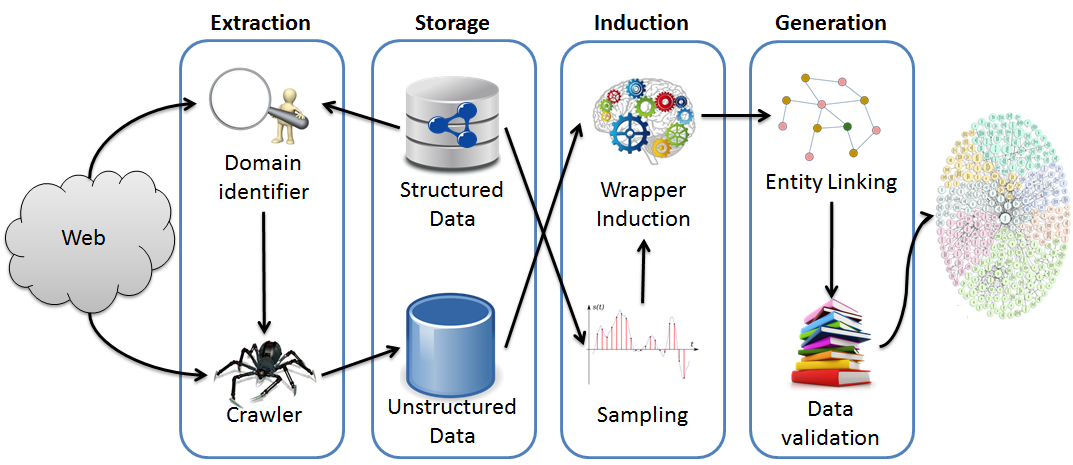
\includegraphics[width = \textwidth]{part_02/semi_structured_annotation/ISWC_REX/rexArchitecture}
\caption{Architecture of REX.}
\label{charex:fig:architecture}
\end{figure}
\subsection{Extraction Layer}
REX's data extraction layer consists of two main components:
The \emph{domain identification module} is the first component of the layer and takes a set of triples $(s, p, o)$ as examples and returns a ranked list of Web domains.
Our current implementation simply uses the Google interface to search for websites that contain the label of all $s$, $p$ and $o$.
The top-10 domains for each triple are selected and their rank is averaged over all triples.
The resulting ranking is returned. 
Moreover, we provide a manual domain identification module for expert users.
For our example \texttt{dbo:actor}, we get \url{http://imdb.com} as top-ranked domain.
The second component consists of a \emph{crawler interface} which allows to gather the Web pages that are part of the detected domain and collect them in a storage solution for unstructured data.
Currently, we rely on crawler4j\footnote{\url{https://code.google.com/p/crawler4j/}} for crawling and Apache Lucene\footnote{\url{http://lucene.apache.org/}} for storing the results of the crawling.  

\subsection{Storage Layer}
The storage layer encapsulates the storage solutions for structured data (i.e., the  \ac{KB} $K$) and the unstructured data (i.e., the output of the extraction layer). 
We assume that the structured data can be access via SPARQL.
The unstructured data storage is expected to return data when presented with a pair $(s, o)$ of resources, which is commonly a positive or negative example for the pairs that abide by $p$.
As stated above, we rely on a Lucene index that can access the labels of resources and simply search through its index for pages that contain both a label for $s$ and a label for $o$.

\subsection{Induction Layer}
The induction layer uses the data in the storage layer to compute wrappers for the website crawled in the first step.
To this end, it contains two types of modules:
The \emph{example generation} module implements sampling algorithms that are used to retrieve examples of relevant pairs $(s, o)$ such that $(s, p, o) \in K$. 
These examples are used to feed the \emph{wrapper induction} module, which learns the wrappers that are finally used to extract data from Web pages.
Hereafter, we present the implementations of these modules.

\subsubsection{Generation of Examples}
Given a  \ac{KB} $K$, the generation of all examples $\examples$ for a predicate $p$ can be retrieved by computing all triples $<s,p,o>$ from $K$.
However, using all triples might lead to poor scalability, especially if $K$ is very large.
To ensure the scalability of our approach, we thus aimed to ensure that we can provide REX with only a sample of $\examples$ and thus reduce its learning runtime without diminishing its accuracy.  
Our first intuition was that it is more likely to find resources that stand for well-known real-world entities on the Web. 
Thus, by selecting the most prominent examples from the knowledge $K$, we should be able to improve the probability of finding Web pages that contain both the subject and the object of our examples. 
This intuition can be regarded as prominence-driven, as it tries to maximize the number of annotated pages used for learning. 
We implemented this intuition to generating a sample of $\examples$ by implementing a first version of the example generator that ranks the examples $(s, o)$ in $\examples$ in descending order by how prominent they are in the  \ac{KB}. The score $scr$ for ranking the examples was computed by summing up the in- and out-degree of $s$ and $o$:
\begin{equation}
scr(s, o) = in(s) + in(o) + out(s) + out(o).
\end{equation}
We call this example selection \emph{prominence-based}.

The main drawback of this first intuition is that it introduces a skew in the sampling as we only consider a subset of entities with a particular distribution across the pages in $W$. 
For example, actors in IMDB have different templates depending on how popular they are. 
Learning only from popular actors would then lead to learning how to extract values only from Web pages obeying to particular type of HTML template. 
%Thus, as our experiments show, while this approach achieves a high recall when looking for web pages, it can lead to incorrect wrappers if only a small subset of $P$ is selected for learning.
%maybe we should write here that the correction of this bias is carried out by the learning appraoch?
While this problem can be by choosing a large number of examples, we revised our sampling approach to still use the ranking but to sample evenly across the whole list of ranked resources. 
To this end, given a number $n$ of required pairs, we return the first $n$ pairs $(s,o)$ from the ranked list computed above whose index $idx$ abides by:
\begin{equation}
idx(s, o) \equiv 0  \left(mod\left \lfloor{\frac{|\examples|}{n}}\right \rfloor \right).
\end{equation}
We call this second implementation of the example generator interface the \emph{uniform} approach .
%By these means, we can ensure that the whole of the distribution of resource prominence is covered by our approach. Consequently, we can support the generation of robust wrappers from the given input data.

%\paragraph{Negative Examples}
%Although it's sufficient to restrict to positive examples only, the usage of negative examples can help to improve the \emph{wrapper induction} step by reducing the hypothesis space. Assuming that we have a positive example $<s,p,o>$ and $dom(p)$(resp. $ran(p)$) denotes the domain (resp. range) of $p$, we generate negative examples as follows:
%\begin{itemize}
%\item Generate a new triple $<s',p,o>$ where $s'$ is an instance of $dom(p)$ and $<s',p,o>$ does not exist in $K$.
%\item Generate a new triple $<s,p,o'>$ where $o'$ is an instance of $ran(p)$ and $<s,p,o'>$ does not exist in $K$.
%\item Generate a new triple $<s',p,o'>$ where $s'$ is an instance of $dom(p)$, $o'$ is an instance of $ran(p)$ and $<s',p,o'>$ does not exist in $K$.
%\end{itemize}


\subsubsection{Wrapper Generation} %(DQ, VC, PM)
\label{alfred}
%- Several approaches in the literature to generate wrappers
%Several years of reasearch on data extraction from web pages have produced a large number of proposals for producing web wrappers (see~\cite{} for a survey). 

% START: alfred commands (Disheng)
\newcommand{\xpath}[1]{\mbox{\sf\small #1}}
%\newcommand{\htmlvalue}[1]{\mbox{\tt\small #1}}
\newcommand{\htmlvalue}[1]{\mbox{`#1'}}
\newcommand{\lc}[2]{\mbox{\ensuremath{LC(#1,#2)}}}%% local consistency
\newcommand{\gc}[2]{\mbox{\ensuremath{Sep(#1,#2)}}}%% global  consistency- separable now!

\newcommand{\allpages}{\mbox{\ensuremath{W}}}
\newcommand{\somepages}{\mbox{\ensuremath{Q}}}
\newcommand{\innersamples}{\mbox{\ensuremath{I}}}
\newcommand{\csample}{\mbox{\ensuremath{C}}}
\newcommand{\nil}[1]{\mbox{\ensuremath{nil_{}}}}
\newcommand{\accr}[1]{\mbox{\ensuremath{Acc(#1)}}}
\newcommand{\vect}[1]{\overrightarrow{#1}}
\newcommand{\rules}{\ensuremath{R}}
\newcommand{\allvects}{\ensuremath{\mathcal{V}^U}}
\newcommand{\allrules}{\ensuremath{\mathcal{R}}}
\newcommand{\nonallrules}{\ensuremath{\overline{\mathcal{R}}}}
\newcommand{\nonammrules}[1]{\ensuremath{\overline{\mathcal{R}}_{#1}}}
\newcommand{\ammvect}[1]{\ensuremath{V_{#1}}}
\newcommand{\ammrule}[1]{\ensuremath{R_{#1}}}
\newcommand{\nonammvect}[1]{\ensuremath{\overline{V}}_{#1}}
\newcommand{\allammrules}[1]{\ensuremath{\mathcal{R}_{#1}}}
\newcommand{\allammvalues}[2]{\ensuremath{\widehat{V}^{#1}_{#2}}}
\newcommand{\queryablevalues}[2]{\ensuremath{V^{#1}_{#2}}(U)}
\newcommand{\lqueryablevalues}[3]{\ensuremath{V^{#1}(#2,#3)}}
\newcommand{\ltypedqueryablevalues}[4]{\ensuremath{V_{#1}^{#2}(#3,#4)}}
\newcommand{\typedqueryablevalues}[2]{\ensuremath{V_{#1}(#2)}}
\newcommand{\equivalence}[1]{\ensuremath{Eq_{U}(#1)}}

\newcommand{\lessexpressive}[1]{\ensuremath{Exp_{min}{(#1)}}}
\newcommand{\equivalencerules}[3]{\ensuremath{Eq^{#3}(#1,#2)}}

\newcommand{\subtypeof}{\ensuremath{\subseteq}}
\newcommand{\supertypeof}{\ensuremath{\supseteq}}

\newcommand{\mq}{\mbox{\em MQ}}
\newcommand{\alf}{\mbox{\sc alf}}
\newcommand{\alfrex}{\mbox{\sc AlfREX}}
\newcommand{\sampler}{{\sc Page\-Sampler}}
\newcommand{\page}{\mbox{\em w}}
\newcommand{\att}[1]{\mbox{\sf #1}}
\newcommand{\val}[1]{{\mbox{\sf '#1'}}}
\newcommand{\valm}[1]{\mbox{\sf #1}}
\newcommand{\abs}[2]{\mbox{\sf abs(#1,#2)}}
\newcommand{\rel}[2]{\mbox{\sf #1(`#2')}}
%\newcommand{\lab}[1]{\mbox{\ensuremath{l(#1)}}}

\newcommand{\alg}[1]{{\sc #1}}
\newcommand{\scegliDomanda}{\textsc{choose\-Question}}
\newcommand{\terminaAlgoritmo}{\mbox{\textsc{halt}}}
\newcommand{\espandiBacinoRegoleCandidate}{\textsc{expandRuleSet}}
\newcommand{\leggiRisposta}{\mbox{\textsc{oracle}}}

\newcommand{\type}[1]{\mbox{\em \ensuremath{#1}}}

\newcommand{\dalvi}{DBLP:journals/pvldb/DalviKS11}
\newcommand{\mdl}{DBLP:journals/corr/math-ST-0406077}
\newcommand{\lixto}{DBLP:conf/pods/GottlobKBHF04}
\newcommand{\angluin}{DBLP:journals/tcs/Angluin04}
\newcommand{\myjacm}{DBLP:journals/jacm/CrescenziM04}
\newcommand{\SL}{DBLP:journals/tnn/Vapnik99}
\newcommand{\srm}{DBLP:journals/tit/Shawe-TaylorBWA98}
\newcommand{\ALsurvey}{settles.tr09}

%\newtheorem{example}{Example}

% END %

%\section{Wrapper Generation}
Detecting rules to extract the subject-object pairs related to a property $p$ is the most difficult step when aiming to extract \ac{RDF} from templated website.
Here, we present our current implementation of the wrapper induction module interface of REX, which aims to extract subject-object pairs for $p$ from a set of pages $\allpages$ that belong to the same website and share a common template.
We assume that an \emph{example generator} provides the input set ${\examples}$ containing a subset of the pairs that can be extracted from the pages in $\allpages$. 
Formally,  let $\somepages$ denote the set of pages that contain a pair in $\examples$:
\begin{equation}
 \somepages = \{\page: \page \in \allpages,\ (s, o)\in {\examples} \wedge (\lab{s},\lab{o}) \in\ \page\},
\end{equation}
where  $(\lab{s},\lab{o}) \in \page$ denotes that at least one of the labels of $s$ and at least one of the labels of $o$ occur in the page $\page$. %In other words, 
We use the pairs in ${\examples}$ to gain the positive annotations for the pages in $\somepages$. These  annotations are needed to automatically infer a set of wrappers, i.e., a set of extraction rule pairs that extract the target subject-object pairs.

%Inferring a wrapper from a large number of annotations increases the computational costs. On the other hand, 
%the accuracy of the generated wrappers strongly depends on the number of training annotations used in the inference process.
%With a small number of annotations, the generated wrappers could be biased towards the variants of the HTML template observable in the sampled pages. For example, if the triples in $\somepages$ are all about famous actors, it might be the case that the inferred rules do not work on pages related to less popular actors in $\allpages$, since these pages could obey a slightly different variant of the template without some fields such as the prizes won, the user comments, etc. etc.

%We introduce a technique that first generate a set of wrappers %starting from a small set of annotations to reduce the costs, and %then rank the wrappers' rules using all the pairs extracted from %$\somepages$ to cover a large
%number of template variants.


% in alternativa alcuni sistemi supervisionati come ALF possono migliorare e certificare la qualità
% la copertura delle regole inferite
To avoid the extraction of incorrect values, our approach includes a technique to evaluate the output wrapper coverage, i.e., the number of pages in {\allpages} for which the wrappers inferred from {\somepages} correctly extract the target subject-object pairs. 

%\subsubsection{Learning Web Wrappers}
%\label{sec:learning-wrappers}

Listing~\ref{lst:learning-wrappers} reports the pseudo-code of our algorithm to generate the wrappers that extract subject-object pairs related to a property $p$ from a set of pages: 
%
it takes as input the set of pages $\allpages$ and the set of examples ${\examples}$.
%, i.e., the pairs $(s,o)$ generated by the previous component, the \emph{example generator}. 
To abstract the extraction rules generative process in our implementation, we assume that there exists, as a parameter of the algorithm, a class of all the creatable extraction rules $\allrules$. It corresponds to the set of XPath expressions that we can generate over the pages in \allpages.

\begin{algorithm}[htb!]
\caption{{\alfrex}: Extract subject-object pairs from a website.}\label{lst:learning-wrappers}
\label{alg:alfrex}
\begin{algorithmic}[1]
\renewcommand{\algorithmicensure}{\textbf{Output:}}
\newcommand{\LET}{\mbox{\textbf{let}}}
\renewcommand{\algorithmicrequire}{\textbf{Input:}}
\REQUIRE \ac{KB} $K$, a predicate $p$, a set of examples $\examples = \{(s,o)|(s,p,o) \in K\}$
\REQUIRE a set of pages $\allpages=\{w_1,\ldots,w_{|\allpages|}\}$ containing data w.r.t. predicate $p$

\renewcommand{\algorithmicrequire}{\textbf{Parameter:}}
\REQUIRE a class of extraction rules $\allrules$ over $\allpages$
\REQUIRE $k$, the number of sample pages for generating the rules

\ENSURE set $T$ of pairs of strings extracted from pages $W$
\bigskip
\STATE $T := \emptyset$; {\em // output pairs of strings}
\STATE $Q := \{\page \in \allpages$: $(\lab{s},\lab{o}) \in \page$, $ (s, o) \in \examples\};$\label{lst:Q}
\STATE $I :=$ a set of $k$ random pages from $Q$;\label{lst:I}
\STATE $R_s := \{r, r \in \allrules, \page \in I, (\lab{s}, \lab{o}) \in \page, r(\page) = \lab{s}\}$;\label{lst:Rs}
\STATE $R_o := \{r, r \in \allrules, \page \in I, (\lab{s}, \lab{o}) \in \page, r(\page) = \lab{o}\}$;\label{lst:Ro}
\STATE $(r_s, r_o) := \argmax_{r_s\in R_s, r_o \in R_o}$~~$|\{\page, \page \in Q, (\lab{s},\lab{o}) \in \page,$\\$ r_s(q) = \lab{s}\ \AND\ r_o(q) = \lab{o}\}|$;\label{lst:best-pair}
\STATE $\{r_s^1,r_s^2,\ldots, r_s^n\} \leftarrow \{r, r \in R_s, r(Q)=r_s(Q) \}$;\label{lst:best-vector-s}
\STATE $\{r_o^1,r_o^2,\ldots, r_o^m\} \leftarrow \{r, r \in R_o, r(Q)=r_o(Q) \}$;\label{lst:best-vector-o}

\FOR{$q\in \allpages$}\label{lst:forall-start}
    \IF {($r_s^1(q)=\ldots=r_s^n(q)\ \AND\ r_o^1(q)=\ldots=r_o^m(q)$)}\label{lst:check}
    \STATE $T \leftarrow T \cup \{(r_s^1(q),r_o^1(q))\}$;
    \ENDIF
\ENDFOR\label{lst:forall-end}

\RETURN $T$;

\end{algorithmic}
\end{algorithm}


As a first step (line~\ref{lst:Q}), the algorithm computes the set of pages $Q$
(we assume $Q \neq \emptyset$).
Then, it picks up a small set of sample pages $I$ from $Q$.%
In our implementation, we set $k = |I| = 10$.
%
From the pages in $I$ two initial sets of extraction rules, $R_s$ and $R_o$, are generated (lines~\ref{lst:Rs}-\ref{lst:Ro}), as follows. 
%
%
First, we analyze the DOM tree of the pages to locate nodes that are part 
of the template. We use these nodes as roots of XPath expressions that 
match with the input pair. To discover the template nodes, we compute the occurrences of the textual leaf nodes in the pages. Following the intuition developed in~\cite{exalg}, 
we consider template nodes the document root, the nodes with an {\em id} attribute, 
and  the text leaves that occur exactly once  with same value and same root-to-leaf sequence of tags in a significant 
percentage (80\%) of pages.  The rationale is that it is very unlikely that a node occurs exactly once in several pages with the same root-to-leaf path by chance; rather, it is likely repeated  in every page since it comes from a piece of the underlying HTML template.

Template nodes are then used as {\em pivot nodes} to generate XPath expressions that 
match with nodes containing a textual leaf that equals the subject (object) of the 
input pair. Given a pivot node $l$, an XPath expression for the textual node $t$ 
is computed by appending three expressions: $(i)$~an expression that matches with the
pivot node $t$, $(ii)$~the path from $t$ to the first ancestor node,
$n_{lt}$, shared by $t$ and $l$, $(iii)$~the path from $n_{lt}$ to $l$ 
(which descends from the shared ancestor node to the target textual node).
To avoid an excessive proliferation of rules, we bound the length of
the XPath expressions, i.e., the number of XPath steps.
We observed that producing rules longer than 8 steps do not produce any benefit.

\begin{figure*}[htb]
\newcommand{\sxpath}[1]{\xpath{\scriptsize#1}}
\begin{tabular}{ccc}
\multicolumn{3}{c}{
\vspace{0pt}
    \resizebox{0.95\textwidth}{!}{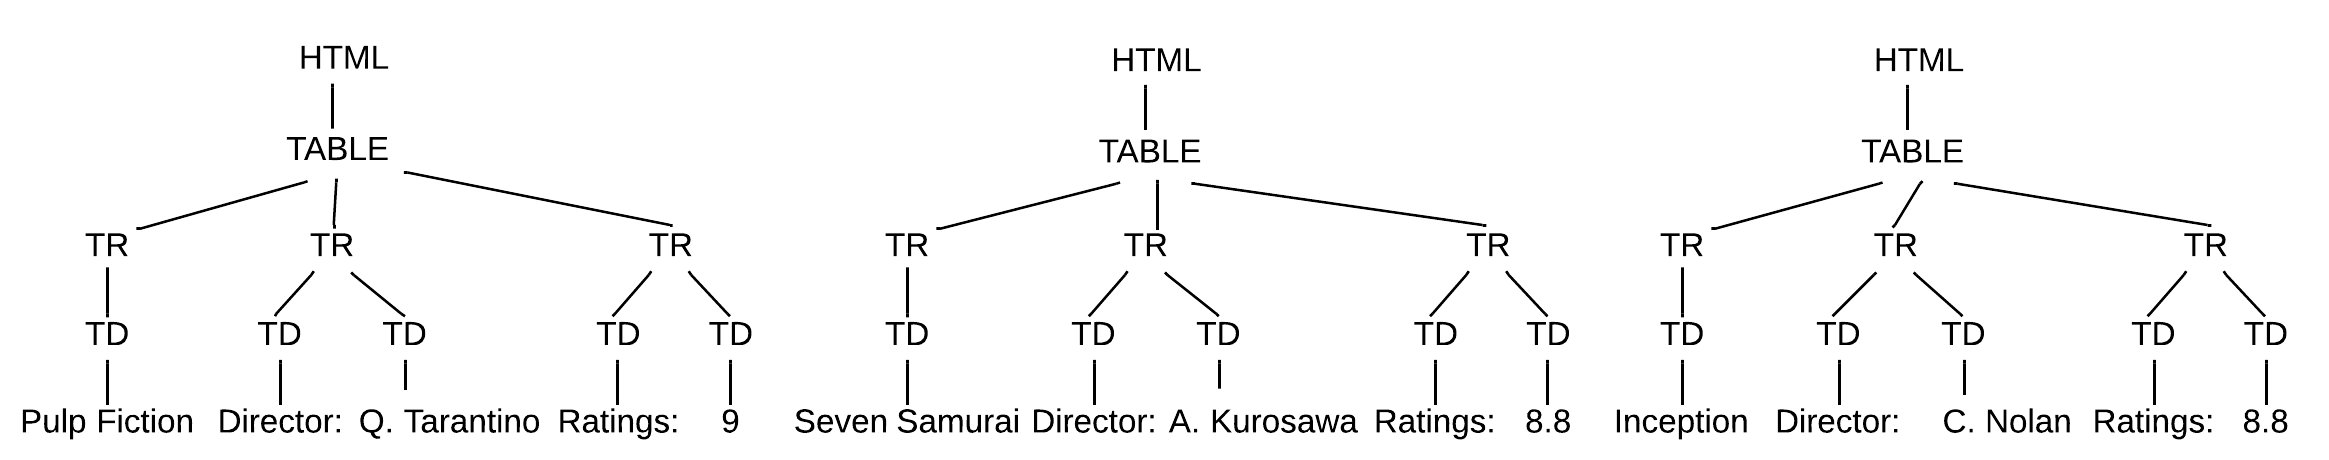
\psfig{file=part_02/semi_structured_annotation/ISWC_REX/dom-I.png}}
}\\
%
\multicolumn{3}{c}{\bf (a)}\\
%
\multicolumn{1}{c}{
    \resizebox{0.2\textwidth}{!}{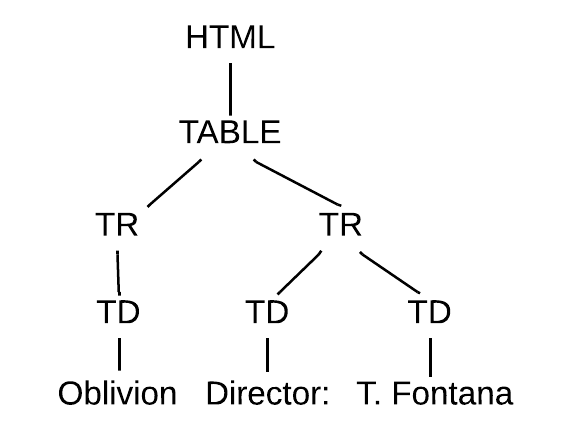
\psfig{file=part_02/semi_structured_annotation/ISWC_REX/dom-Q.png}} 
} &
\multicolumn{1}{@{}c@{}}{
    \raisebox{0.5\totalheight}{
    \scalebox{0.85}{
\begin{tabular}{@{}r@{:~}l@{}}
\multicolumn{2}{l}{\em Extraction rules}\\
$r^1$  & {\sxpath{//*[contains(.,"Ratings:")]/../p-s::tr[2]/td/text()
}}\\
$r^2$  & {\sxpath{//*[contains(.,"Director:")]/../p-s::tr[1]/td/text()
}}\\
$r^3$  & {\sxpath{/html/table/tr[1]/td/text()}}\\
\multicolumn{2}{l}{\em ps = preceding-siblings} \\
\end{tabular}}}}  &
\vspace{0pt}
    \resizebox{0.35\textwidth}{!}{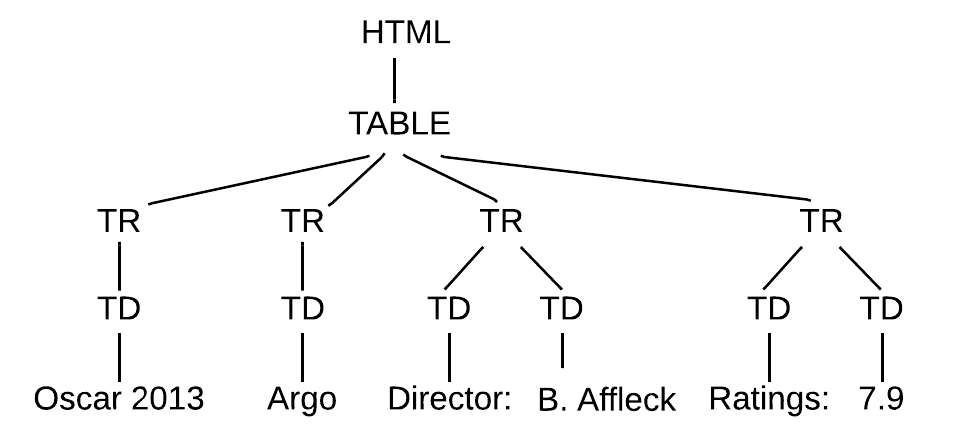
\psfig{file=part_02/semi_structured_annotation/ISWC_REX/dom-W.png}} \\
%
\multicolumn{1}{c}{\bf (b)} & \multicolumn{1}{c}{\bf (c)} & \multicolumn{1}{c}{\bf (d)} 
\\
\end{tabular}
 \caption{%
 {\bf (a)} DOM trees of three pages (in a fictional set $I$), 
 {\bf (b)} a page in $Q$ (with a template that differs from those of the pages in $I$), 
 {\bf (c)} some rules to extract the movie title, and
 {\bf (d)} a page in $W$ (with a template that differs from those of the pages in $Q$).}%
 \label{fig:dom-trees}
\end{figure*}


The above step produces several extraction rules that correctly work on the pages 
in $I$. However some of these rules could not work on a larger set of pages. 
For example, consider a set of pages such as those shown in Figure~\ref{fig:dom-trees} (a). Assuming that the leaf nodes {\htmlvalue{Director:}} and {\htmlvalue{Ratings:}} appear once with the same root-to-leaf path in most of the pages in $I$, they would be considered as template nodes. Figure~\ref{fig:dom-trees} (c) reports an example of the XPath expressions pivoted in these nodes, and generated to extract the movie title.
%
%\end{example} 
%
Notice, however, that rule $r^1$ does not extract the movie title on pages like that depicted in Figure~\ref{fig:dom-trees} (b), i.e., pages without user ratings.
To improve the accuracy of the rules generated from pages in $I$, we evaluate the generated rules over $Q$, and select those that extract the largest number of annotations (line~\ref{lst:best-pair}). In our example, the extraction rules $r^2$ and $r^3$ would be selected, while $r^1$ would be discarded, as the former rules work also on the page of Figure~\ref{fig:dom-trees} (b), while the latter does not. 

%\floatname{algorithm}{Listing}



The selected rules are those better working for the pages in $Q$, that are the pages containing pairs of $K$. Although it is likely that these rules also work for the whole collection of input pages, it might also be the case that {\allpages} contains pages obeying to a slightly different template not observed within $Q$. For example, consider the page in Figure~\ref{fig:dom-trees} (d): since the movie has been awarded 3 Oscars, the corresponding page has small structural differences, and neither $r^1$ nor $r^3$ correctly extract the title. 


To overcome this issue, we leverage the redundancy of equivalent rules generated in the above steps. Targeting only resources from pages for which the extraction is likely to work correctly, we return the pairs (lines~\ref{lst:best-vector-s}-\ref{lst:best-vector-o}) on which all the distinct yet equivalent rules return the same value. Again from our example, observe that rules $r^2$ and $r^3$ extract different values from the page in Figure~\ref{fig:dom-trees} (d) ({\em Argo} and {\em Oscar 2013}, respectively), therefore, none of the values extracted from that page would be added in the final output. 
%{\bf DQ: cosi funziona? :)}
%{\bf DA SISTEMARE. ATTENZIONE: L'ESEMPIO NON FUNZIONA LE DUE REGOLE SI COMPORTANO ALLO STESSO MODO}
All these rules are used later (lines~\ref{lst:forall-start}-\ref{lst:forall-end}) to check that they extract the same value (line~\ref{lst:check}) from a web page.


%We could also rely to other supervised systems (such as~\cite{DBLP:conf/www/CrescenziMQ13a}) to further improve and guarantee the quality and the coverage of the extraction rules.



\subsection{Generation Layer}
Now that data has been extracted from the websites, REX is ready to generate \ac{RDF} out of them. 
To achieve this goal, two steps needs to be carried out. 
First, the strings retrieved have to be mapped to \ac{RDF} resources or literals. 
This is carried out by the \emph{URI disambiguation} modules. 
The resulting triples then need to be checked for whether they go against the ontology of the  \ac{KB} or other consistency rules. 
This functionality is implemented in the \emph{data validation} modules. 

\subsubsection{URI Disambiguation}\label{urigen}
%Subsequently to generating the best possible wrapper for a domain of a property $p$ we need to generate triples from each pair $(s, o) \in T$.
%To achieve this goal, we try to match $(s,o)$ against resources from the knowledge base $K$.
URI disambiguation is not a trivial task, as several resources can share the same label in a  \ac{KB}. 
For example, ``Brad Pitt'' can be mapped to the resource \texttt{:Brad\_Pitt} (the movie star) or \texttt{:Brad\_Pitt\_(boxer)}, an Australian boxer. 
We address this problem by using \emph{AGDISTIS}, a framework for URI disambiguation~\cite{agdistis_iswc}.
In our current implementation, we chose to simply integrate the AGDISTIS framework using DBpedia 3.8.
We chose this framework because it outperforms the state-of-the-art frameworks AIDA~\cite{AIDA} and DBpedia Spotlight~\cite{spotlight} by 20\% w.r.t. its accuracy. 
Especially on short RSS feeds containing only two resource labels, the approach achieves 3\%  to 11\% higher accuracy. 
More details on AGDISTIS as well as a thorough evaluation against popular frameworks such as DBpedia Spotlight and AIDA can be found in~\cite{agdistis_iswc}.
Note that if no resources in $K$ has a URI which matches $s$ or $o$, we generate a new cool URI\footnote{\url{http://www.w3.org/TR/cooluris}} for this string.% following the DBpedia guidelines~\cite{DBLP:conf/semweb/AuerBKLCI07}.

\subsubsection{Data Validation}\label{axioms}
Sequentially applying the steps before results in a set of triples $<s,p,o>$ that might not be contained in $K$. 
As we assume that we start from a consistent  \ac{KB} $K$ and the whole triple generation process until here is carried out automatically, we need to ensure that $K$ remains consistent after adding $<s,p,o>$ to $K$.
To this end, REX provides a data validation interface whose first implementation was based on the DL-Learner.\footnote{\url{http://dl-learner.org}}
Depending on the size of $K$, using a standard OWL reasoner for consistency checks can be intractable.
%\todo[inline]{@Lorenz: Citation for the claim pls}
Thus, our current implementation applies the following set of rules based on the schema of $K$ and add a triple $<s_1,p,o_1>$ only if it holds that:
\begin{enumerate}
\item If a class $C$ is the domain of $p$, there exists no type $D$ of $s_1$ such that $C$ and $D$ are disjoint.
\item If a class $C$ is the range of $p$, there exists no type $D$ of $o_1$ such that $C$ and $D$ are disjoint.
\item If $p$ is declared to be functional, there exists no triple $<s_1,p,o_2>$ in $K$ such that $o_1 \neq o_2$.
\item If $p$ is declared to be inverse functional, there exists no triple $<s_2,p,o_1>$ in $K$ such that $s_1 \neq s_2$.
\item If $p$ is declared to be asymmetric, there exists no triple $<o_1,p,s_1>$ in $K$.
\item If $p$ is declared to be irreflexive, it holds that $s_1 \neq o_1$.
\end{enumerate}
Note that this approach is sound but of course incomplete.
Although an increasing number of \ac{RDF}  \ac{KB}s are published, many of those consist primarily of instance data and lack sophisticated schemata. 
To support the application of the above defined rules, we follow the work in \cite{buhmann2012,pattern_enrichment}, which provides a lightweight and efficient schema creation approach that scales to large  \ac{KB}s. 
%The creation of the (extended) schema is done in three steps:

%\begin{enumerate}
%\item In the optional first step, SPARQL queries are used to obtain existing information about the schema of the  \ac{KB}, in particular we retrieve axioms which allow to construct the class hierarchy. Naturally, the schema only needs to be obtained once per  \ac{KB} and can then be re-used by all algorithms and all entities.
%\item The second step consists of obtaining all the data via SPARQL, which is relevant for learning the considered axiom.
%This results in a set of axiom candidates.
%\item In the third step, the score of axiom candidates is computed and the results returned.
%\end{enumerate}

%Suppose we want to search for the domain of $p$ and got a class $A$ as possible candidate from step 2, then we have to run 3 SPARQL queries to obtain all data for computing the score by means of precision and recall: one query for the number of instances having at least one $p$ ($|\exists p.\top|$), one for the instance count of $A$ ($|A|)$, and another one to get the number of instances contained in the intersection of both ($|\exists p.\top \sqcap A|$).
%Based on that information, we can compute precision $P$ as $P=\frac{|\exists p.\top \sqcap A|}{|A|}$ and recall $R$ as $R=\frac{|\exists p.\top \sqcap A|}{|\exists p.\top|}$, both resulting in a total score for  $A$  being the domain of $p$ using standard F-measure.

%A disadvantage of using this straightforward method of obtaining a score is that it does not take the \emph{support} for an axiom in the  \ac{KB} into account. 
%Specifically, there would be no difference between having 100 out of 100 correct observations or 3 out of 3 correct observations when computing precision and recall.
%For this reason, we do not just consider the count, but the average of the 95\% confidence interval of the count.
%This confidence interval can be computed efficiently by using the improved Wald method defined in~\cite{approx}. 
%Assume we have $\mu$ observations out of which $\sigma$ were successful, then the approximation of the 95\% confidence interval is as follows:

%\begin{scriptsize}
%\[
%\left[
% \max(0, p' - 1.96 \cdot \sqrt{\frac{p' \cdot (1-p')}{\mu+4}}) , %\textnormal{ to }
% \min(1, p' + 1.96 \cdot \sqrt{\frac{p' \cdot (1-p')}{\mu+4}}) 
%\right]
%\]
%\end{scriptsize}

%\noindent
%with $p' = \frac{\sigma+2}{\mu+4}$.
%This formula is easy to compute and has been shown to be accurate in~\cite{approx}.
%This step concludes the extraction of RDF triples from websites.

\section{Evaluation}
\label{sec:evaluation}
The goal of the evaluation was to provide a detailed study of the behavior of the current REX modules with the aim of (1) ensuring that our framework can be used even in its current version and (2) detecting current weaknesses of our framework to trigger future developments.
In the following, we begin by presenting the data and hardware we used for our experiments. 
Thereafter, we present and discuss the results of our experiments.
Detailed results can be found at the project website.

%\begin{enumerate}

%\item We wanted to determine the amount of knowledge that we need to learn sensible pairs of XPath expressions. We thus provided our wrapper inference component with a variable number of examples and measured the influence of the number of examples on the overall F-measure of our approach. 
%%\item We also wanted to evaluate how well our approach can estimate its own confidence in the expressions it learned. We thus conducted a series of experiments where we measured the change in sure of our approach with varying confidence thresholds.
%\item To measure the runtime performance of our approach, we measured the amount of time that REX required to learn  wrappers from the input data. Especially, we measures the influence of the size of $I$ on the runtime of REX as well as on the average F-measure achieved by our approach. 
%\item Finally, we wanted to measure the quality of the end result of our approach, i.e., the quality of the output RDF. We thus sampled the triples generated by our approach and approximated its overall accuracy. 
%\end{enumerate}
 
\subsection{Experimental Setup}
We generated our experimental data by crawling three websites, i.e., 
\begin{enumerate}
\item \url{imdb.com} where we extracted \url{dbo:starring}, \url{dbo:starring}$^{-1}$ as well as \url{dbo:director};
\item \url{goodreads.com}, from which we extracted \url{dbo:author} and \url{dbo:author}$^{-1}$;
\item \url{espnfc.com} with the target relations \url{dbo:team} and \url{dbo:team}$^{-1}$.
\end{enumerate}
%For each website, we focused on two subdomains (see~Table~\ref{tab:dataset}). 
We chose these websites because they represent three different categories of templated websites.
\url{imdb.com} widely follows a uniform template for all pages in the same subdomain.
%Moreover, there are rarely any pages with missing values in this site.
Thus, we expected the wrapper learning  to work well here.
\url{goodreads.com} represents an average case of templated websites. 
While template are most widely used and followed, missing values and misused fields are more common here than in our first dataset.
%Thus, we assume that the values achieved on this dataset can be regarded as prototypical for our approach.
The third dataset, \url{espnfc.com}, was chosen as worst-case scenario.
The dataset contains several blank pages, a large variety of  templates used in manifold different fashions.
Consequently, defining a set of golden XPaths is a tedious task, even for trained experts.
Thus, we expected the results on this dataset to be typical for the worst-case behavior of our approach.
%Since all domains support incremental URLs we randomly sampled valid numbers in the respective range of valid URLs. 
We randomly sampled 10,000 HTML pages per subdomain for our experiments and manually built reference XPath expressions to evaluate the precision and recall of the generated extraction rules. 
The precision, recall and F-measure reported below were computed by comparing the output of REX with the output of the reference XPath expressions.
All extraction runtime experiments were carried out on single nodes of an Amazon EC2.small instance.

%\todo[inline]{State that some of the used properties are uni-directional}
%\todo[inline]{In the paper of \cite{Crescenzi2013} a much more sophisticated crawling strategy is described. We could engage this by stating that we crawl a much higher amount of data without loosing web-scalability}


%\begin{table}[htb]
%\centering
%\caption{Properties per dataset. \texttt{dbo} stands for \texttt{http://dbpedia.org/ontology/}.} 
%\label{tab:dataset}
%\begin{tabular}{lll}
%\toprule
%%\multicolumn{2}{c}{Domain}&Property\\
%%\midrule
%\multirow{2}{*}{\url{goodreads.com}} & Author   & \url{dbo:author}$^{-1}$\\
%                                     & Book     & \url{dbo:author} \\
%\midrule
%\multirow{2}{*}{\url{espnfc.com}}    & Team     & \url{dbo:team}$^{-1}$\\
%                                     & Player   & \url{dbo:team} \\
%\midrule
%\multirow{2}{*}{\url{imdb.com}}      & Actor    & \url{dbo:starring}$^{-1}$ \\
%                                     & Movie    & \url{dbo:starring} \\
%                                      & Movie    & \url{dbo:director} \\
%\bottomrule
%\end{tabular}
%\end{table}

\subsection{Results}
\paragraph{Effect of Number of Examples and Sampling Strategy on F-measure}


%\todo[inline]{RU: I think we need to define which f-measure was used here. AN: Done}
The results of our experiments on altering the number of examples used for learning are shown in Figures~\ref{charex:fig:pDirector}-\ref{charex:fig:uTeam}. 
Due to space limitations, we show the average results over all the pairs extraction by our wrapper induction approach for each of the domains.
The results achieved using the prominence-based sampling show the expected trend: on pages that use a consistent template (such as the director pages in \url{imdb.com}), our approach requires as few as around 70 pages for $|Q|$. 
Once this value is reached, REX can compute high-quality extraction rules and achieves an F-measure of 0.97 (see Figures~\ref{charex:fig:pDirector}).
For pages that change template based on the prominence of the entities they describe (like the actors' pages, see Figure~\ref{charex:fig:pActors}), our approach requires more training data to achieve a high F-measure.
The increase of F-measure is clearly due to an increase in precision, pointing to REX being able to better choose across different alternative XPaths when provided with more information.
The results of \url{goodreads.com} support our conjecture. 
With more training data, we get an increase in precision to up to 1 while the recall drops, leading to an overall F-measure of 0.89 for 40.000 examples.
In our worst-case scenario, we achieve an overall F-measure close to 0.6.
The lower value is clearly due to the inconsistent use of templates across the different pages in the subdomains.


\begin{figure}[htb!]
        \centering
        \subfloat[Directors from IMDB, prominence-based sampling.]{\label{charex:fig:pDirector}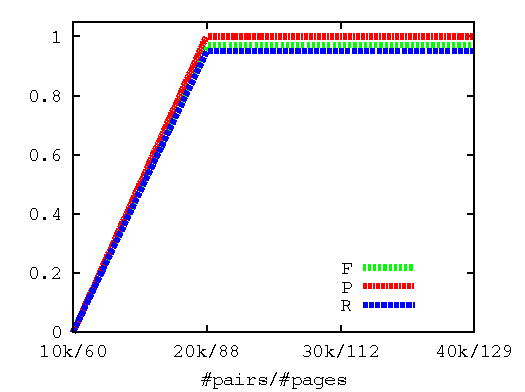
\includegraphics[width=.33\textwidth]{part_02/semi_structured_annotation/ISWC_REX/no-random-director.pdf}}~
        \subfloat[Actors from IMDB, prominence-based sampling.]{\label{charex:fig:pActors}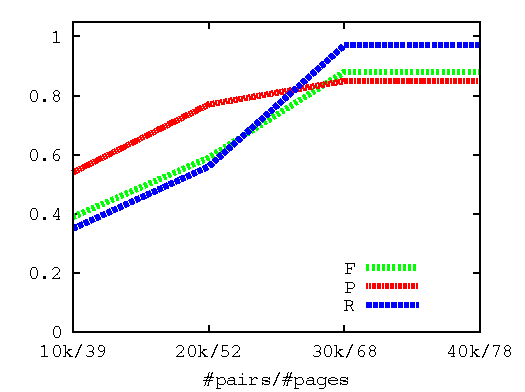
\includegraphics[width=.33\textwidth]{part_02/semi_structured_annotation/ISWC_REX/no-random-starring.pdf}}~
        \subfloat[Authors from Goodreads, prominence-based sampling.]{\label{charex:fig:pAuthor}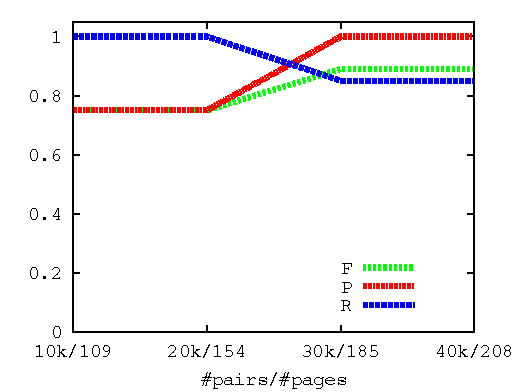
\includegraphics[width=.33\textwidth]{part_02/semi_structured_annotation/ISWC_REX/no-random-author.pdf}}

        \subfloat[Directors from IMDB, uniform sampling.]{\label{charex:fig:uDirector}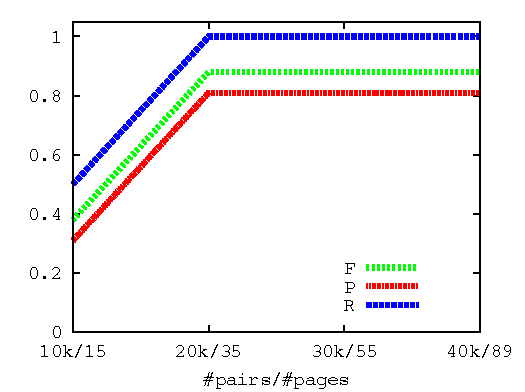
\includegraphics[width=.33\textwidth]{part_02/semi_structured_annotation/ISWC_REX/random-director.pdf}}~
        \subfloat[Actors from IMDB, uniform sampling.]{\label{charex:fig:uActors}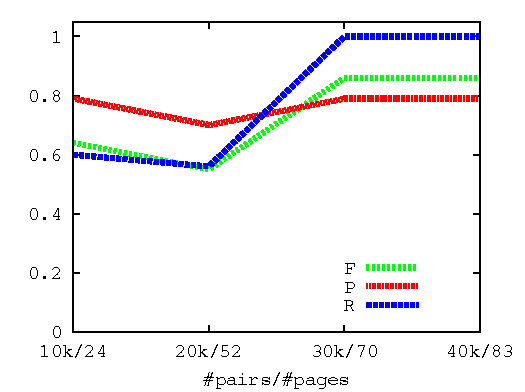
\includegraphics[width=.33\textwidth]{part_02/semi_structured_annotation/ISWC_REX/random-starring.pdf}}~
        \subfloat[Authors from Goodreads, uniform sampling.]{\label{charex:fig:uAuthor}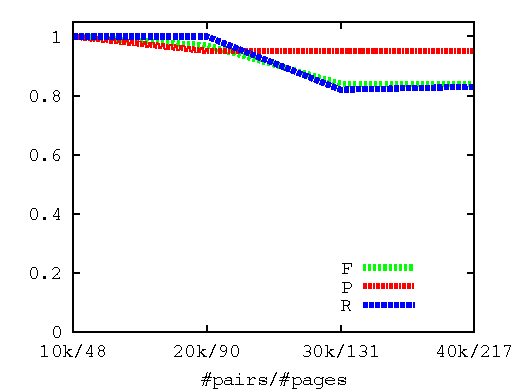
\includegraphics[width=.33\textwidth]{part_02/semi_structured_annotation/ISWC_REX/random-author.pdf}}
        
        \subfloat[Teams from ESPNFC, prominence-based sampling.]{\label{charex:fig:pTeam}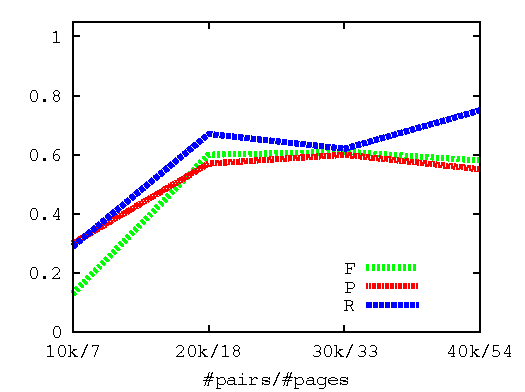
\includegraphics[width=.33\textwidth]{part_02/semi_structured_annotation/ISWC_REX/no-random-team.pdf}}~
        \subfloat[Teams from ESPNFC, uniform sampling.]{\label{charex:fig:uTeam}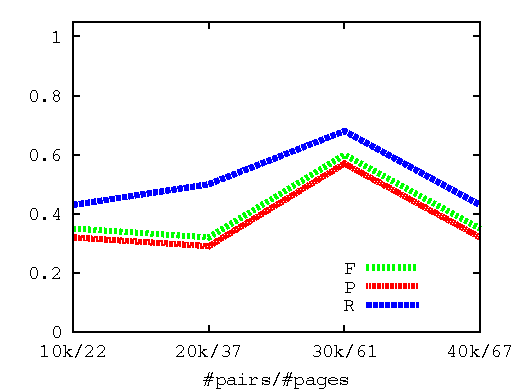
\includegraphics[width=.33\textwidth]{part_02/semi_structured_annotation/ISWC_REX/random-team.pdf}}~
        \subfloat[Average computational time and F-measure over all datasets.]{\label{charex:fig:runtime}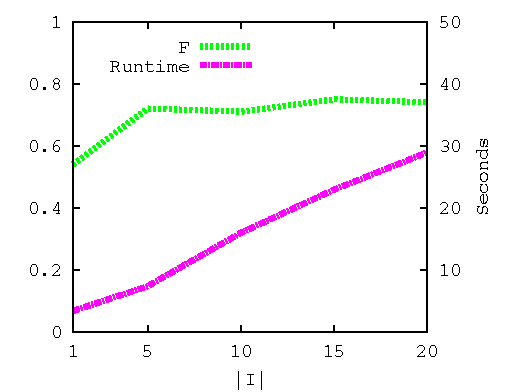
\includegraphics[width=.33\textwidth]{part_02/semi_structured_annotation/ISWC_REX/time-F.pdf}}
\caption[Overall evaluation results of REX]{Overall evaluation results of the extraction of pairs. Figures (a) to (h) show the average precision, recall and F-measure which is achiev\-ed by the generated XPaths for the prominence-based and uniform sampling. The x-axis shows the number of examples and the number of sample pages retrieved in the format $|E|$/$|Q|$. Figure (i) shows the average computational time and the corresponding F-measures for different sizes of $|I|$.}
\label{charex:fig:overall-XPaths}
\end{figure}


The results based on the uniform sampling strategy reveal another trait of REX. 
As expected, the coverage achieved using uniform sampling is clearly smaller in all cases. 
%Still, when a small number of examples $|E|$ is provided, the uniform sampling returns better results than the prominence-based sampling (compare results with $|E| = 10k$ on Figures~\ref{charex:fig:pDirector} and~\ref{charex:fig:uDirector}, Figures~\ref{charex:fig:pActors} and~\ref{charex:fig:uActors}, Figures~\ref{charex:fig:pAuthor} and~\ref{charex:fig:uAuthor} as well as Figures~\ref{charex:fig:pTeam} and~\ref{charex:fig:uTeam}) in all settings.  
%This is simply due to the examples selected by the uniform sampling better reflecting the different types of templates in the dataset.
%The main drawback of the uniform sampling strategy is that the instances it selects generally contain a larger percentage of erroneous resources than the data selected by the prominence-based sampling strategy.
%The effect of this larger percentage of erroneous resources increases when making use of larger sizes of uniformly %sampled examples $E$ if the fraction of pages with noisy data in $Q$ increases.
%With a larger percentage of noise in the training data, REX is then more prone to learn biased and sub-optimal XPath expressions, leading to the overall decrease of the F-measure of our system.
%The proportion of erroneous pages in the training data is yet different from dataset to dataset, leading to different patterns combing about across our experiments. For example, extracting teams already leads to more errors in the uniform sampling when $|E| = 20k$ while the precision remains superior for $|E| = 20k$ when extracting author data from \url{goodreads.com}. 
%Our observations led us to the following conclusions: When running (1) on a manually curated  \ac{KB} with only a small amount of erroneous data in the  \ac{KB} or (2) on a small number of examples $|E|$, the uniform distribution is to be preferred.
%However, when running on an automatically extracted  \ac{KB} or on a large set of examples, the prominence-based distribution should be used.
%An exact quantification of this behavior remains part of our future work.
The results achieved with all the training data available clearly show the importance of sampling, see Table~\ref{tab:overall}. 
While one could conjecture that using all data for training would be beneficial for our approach, the F-measures achieved by using all the data suggest that sampling can be beneficial for the extraction, especially when the Web pages do not follow a rigid template, e.g., in \url{esnpfc.com}, or when the data in the  \ac{KB} is noisy. 
Overall, our results suggest that our approach is accurate, also for pages where entities with different prominence are assigned variable templates as in \url{imdb.com} actors. 
If multiple occurrences of the same value are present in the same page (as in the case of books, actors and directors), our algorithm is able to detect the most stable one.
Moreover, our approach seems robust against noisy labels, even when there are many false positive in the page (e.g., book author pages that include many links to different books by the same author).
An important feature of our approach is that it can obtain accurate XPaths even by learning from a very small fraction of pages. 
For example, in our experiments on up to 40.000 pages, our approach learned XPath expressions from only 0.5\% to 1.16\% of $|W|$.
Still, for very noisy domains with an inconsistent use of templates, our approach can lead to less accurate extraction rules.
%, as shown by our results on the third dataset.
%Yet, manually crafting XPath expressions to extract these data is a very tedious task.
\begin{table}[htb]
\centering
\begin{tabular}{lcccc}
\toprule
  &  P & R & F-measure & \#Pages \\
\midrule
\url{dbo:director}  & 0.82 & 1.00 & 0.89 & 216\\
\url{dbo:starring}  & 0.86 & 1.00 & 0.90 & 316\\
\url{dbo:author}    & 0.94 & 0.85 & 0.86 & 217\\
\url{dbo:team}      & 0.32 & 0.43 & 0.35 & 656\\
\bottomrule
\end{tabular}
\caption{Average evaluation results using all available pairs as training data.} 
\label{tab:overall}
\end{table}

\paragraph{Runtime Performance}
We evaluated the runtime performance of our approach by using 40.000 examples and the prominence-based distribution while altering the size of $I$. 
As expected, setting $|I|$ to a low value, e.g.,~1, leads to less rules being generated and thus to an overall better runtime performance, see~Figure~\ref{charex:fig:runtime}.
By setting $I$ to a low value, REX can be used to get a quick overview of possible extraction results, a
characteristic of our system that could result beneficial for end users.
Yet, it also leads to worse overall F-measures.
Setting $I$ to a higher value, e.g., 15, leads to a more thorough, i.e., more time-demanding, analysis of the websites and thus to better results. 
Still overall, our approach scales quasi linearly and requires on average less than thirty seconds to learn wrappers out of existing data even for $|I|=20$.

\paragraph{Quality of RDF Output}
To check the quality of the \ac{RDF} we generated, we manually checked the triples extracted from each property of our three domains.
Each triple was checked by at least two annotators, which reached a significant Kohen's kappa score~\cite{cohen1960coefficient} of 0.88 overall.
On \url{goodreads.com} we achieved a precision of 75.24\%.
While we achieve a precision of 78.85\% when extraction directors from \url{imdb.com} and of 75\% on \texttt{starring}, the extraction of \texttt{starring}$^{-1}$ proves more tedious (precision = 42.17\%).
As expected, the data extracted from \url{espnfc.com} has a low precision of 44.19\%.
The results on \texttt{starring}$^{-1}$ are due to the fact that several actors can star in a movie while assuming other roles. 
Thus, our extraction framework often overgenerates triples and produces false positives, e.g., directors are often included.
The results on \url{espnfc.com} are clearly due to the templates not being used correctly.
Still, our results clearly show the potential of our approach, as 60.68\% of the triples we extracted are both correct and novel, see Table~\ref{tab:rdfeval}.


\begin{table}[htb!]
\centering
\resizebox{\textwidth}{!}{ 
\begin{tabular}{lccccc}
\toprule
Property & \#Possible & \#Triples generated & \#Consistent & \#Correct & \#New   \\
 & triples   & by AlfREX& triples & triples & triples  \\
\midrule 
\url{dbo:author}$^{-1}$   & 54 & 32 & 32 & 22 & 22 \\% (67.7\%)\\
\url{dbo:author}          & 83 & 83 & 69 & 54 & 54 \\%(77.0\%)\\
\midrule 
\url{dbo:team}$^{-1}$     & 2  & 1  & 1  & 0  & 0  \\%(0\%)\\
\url{dbo:team}            & 30 & 55 & 42 & 19 & 13\\ %90 & 50 & ? & ? \\%(31.0\%) \\
\midrule 
\url{dbo:starring}$^{-1}$ & 40 & 99 & 83 & 35 & 34 \\%(42.7\%)\\
\url{dbo:starring}        & 70 & 70 & 44 & 33 & 32 \\%(73.9\%)\\
\midrule
\url{dbo:director}        & 61 & 56 & 52 & 41 & 41 \\%(78.8\%)\\
\bottomrule
\end{tabular} }
\caption{Triples generated by 100 randomly sampled pages, number of possible triples generated by using gold standard rules}
\label{tab:rdfeval}
\end{table}
